\documentclass[11pt,a4paper]{article}
\usepackage[utf8]{inputenc}
\usepackage[margin=1in]{geometry}
\usepackage{graphicx}
\usepackage{tikz}
\usepackage{float}
\usepackage{tabularx}
\usepackage{hyperref}
\usepackage{xcolor}
\usepackage{listings}
\usepackage{fancyhdr}
\usepackage{multicol}

\usetikzlibrary{shapes.geometric, arrows, positioning, fit, backgrounds, shadows}

\tikzstyle{system} = [rectangle, rounded corners, minimum width=3cm, minimum height=1cm, text centered, draw=black, fill=gray!30, drop shadow]
\tikzstyle{component} = [rectangle, minimum width=2.5cm, minimum height=0.8cm, text centered, draw=black, fill=blue!10]
\tikzstyle{database} = [cylinder, shape border rotate=90, aspect=0.3, minimum width=2.5cm, minimum height=1.2cm, text centered, draw=black, fill=green!20]
\tikzstyle{external} = [rectangle, minimum width=2.5cm, minimum height=0.8cm, text centered, draw=black, fill=orange!20]
\tikzstyle{process} = [rectangle, minimum width=2.5cm, minimum height=0.8cm, text centered, draw=black, fill=green!10]
\tikzstyle{decision} = [diamond, aspect=2, minimum width=2cm, minimum height=0.8cm, text centered, draw=black, fill=yellow!20]
\tikzstyle{arrow} = [thick,->,>=stealth]
\tikzstyle{line} = [thick,-]

\pagestyle{fancy}
\fancyhf{}
\rfoot{\thepage}

\title{\textbf{Case-Event-Relay Technical Report}}
\author{}
\date{}

\begin{document}

\maketitle

\section*{Executive Summary}

The Case-Event-Relay is a critical infrastructure service in Datadog's case management domain that implements the transactional outbox pattern to ensure reliable event delivery from PostgreSQL to Kafka. It acts as a bridge between the Case Management database and the event streaming platform, reading domain events from the \texttt{domain\_event} table and publishing them to Kafka topics for consumption by downstream event handlers. The service uses an active-passive deployment model with distributed locking to prevent duplicate event delivery while maintaining high availability through automatic failover.

\section{Service Overview}

\subsection{Primary Functions}

\begin{enumerate}
    \item \textbf{Event Relay}: Reads unread domain events from PostgreSQL and publishes them to Kafka topics
    \item \textbf{Outbox Pattern Implementation}: Ensures reliable event delivery through transactional storage before Kafka publication
    \item \textbf{Distributed Lock Management}: Maintains exclusive processing lock across multiple replicas using active-passive pattern
    \item \textbf{Event Acknowledgment}: Tracks Kafka delivery confirmations and removes acknowledged events from the database
    \item \textbf{Backlog Monitoring}: Continuously reports unread event counts for observability and alerting
    \item \textbf{Corrupt Event Isolation}: Identifies and marks corrupt events to prevent pipeline blocking
\end{enumerate}

\subsection{Key Characteristics}

\textbf{Deployment Model}
\begin{itemize}
    \item Active-Passive: Single active pod processes events at any time
    \item Distributed Lock: Uses PostgreSQL table for coordination across replicas
    \item Automatic Failover: Lock acquisition timeout of 20 seconds for pod failure recovery
    \item Lock Heartbeat: 10-second interval to maintain ownership
\end{itemize}

\textbf{Performance Configuration}
\begin{itemize}
    \item Polling Period: 250ms between database reads
    \item Batch Size: Up to 1000 events per read cycle
    \item Ack Batch Size: Up to 1000 events deleted per acknowledgment cycle
    \item Ack Cycle: 20ms tick for responsive acknowledgment processing
    \item Kafka Partitions: 32 partitions for parallel downstream processing
\end{itemize}

\subsection{Key Metrics}

\begin{itemize}
    \item \textbf{Replicas}: 1 per datacenter (active-passive via lock)
    \item \textbf{Resource Allocation}: 1 CPU core, 1-2Gi memory
    \item \textbf{Throughput}: Handles thousands of events per second
    \item \textbf{Latency}: Typically sub-second from database write to Kafka delivery
    \item \textbf{Topics Produced}: domain-events (Case Management), domain-events-oncall (On-Call)
    \item \textbf{Event Types}: 60+ domain event types (case lifecycle, assignments, integrations, etc.)
    \item \textbf{Deployment Environments}: Staging, Production, Government (FIPS-compliant)
\end{itemize}

\section{Architecture Overview}

\subsection{System Architecture}

The case-event-relay service sits between the Case Management database and Kafka, implementing a reliable event relay pattern. It reads events from a transactional outbox table, publishes them to Kafka, and removes them only after delivery confirmation.

\clearpage

\begin{figure}[H]
\centering
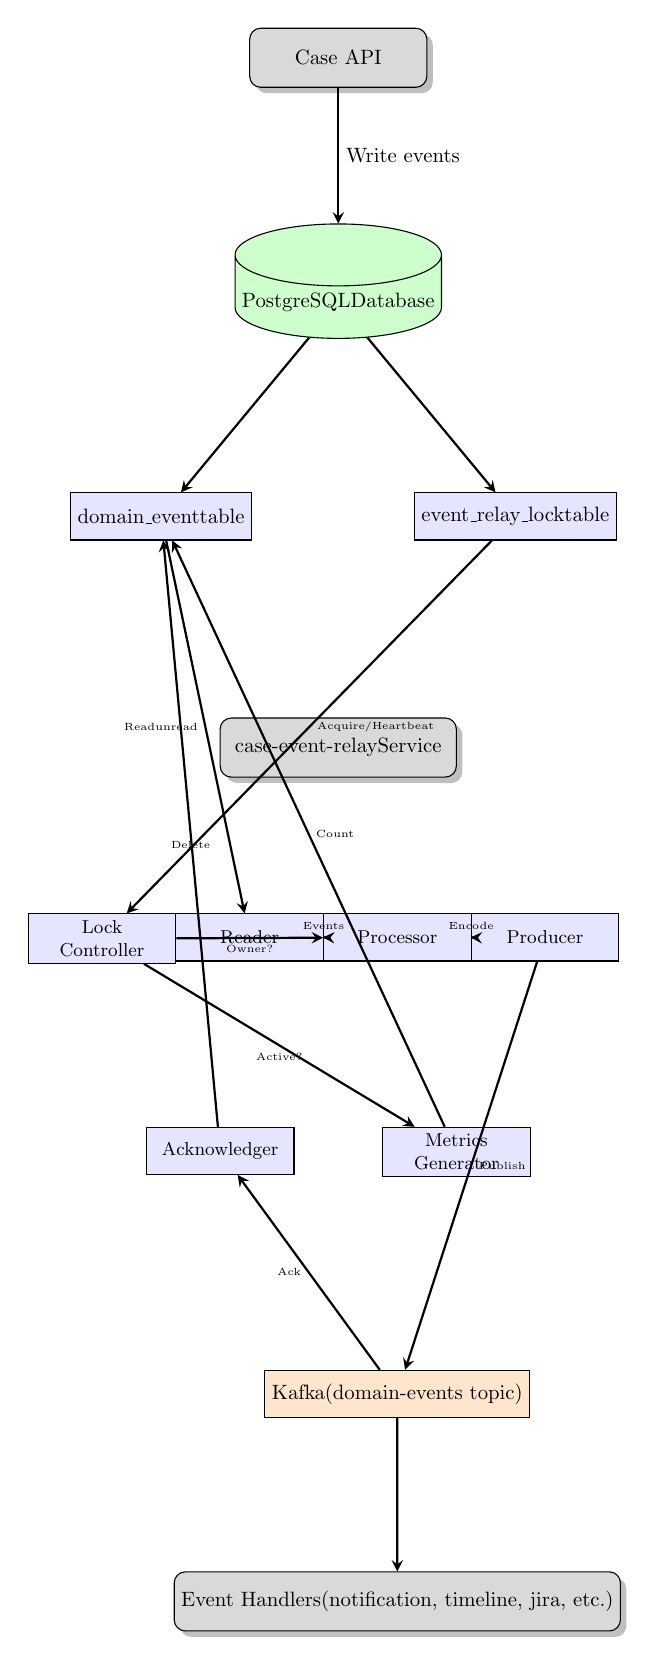
\begin{tikzpicture}[node distance=1.8cm, scale=0.75, every node/.style={transform shape}]

% Case API (writes events)
\node (case-api) [system] {Case API};

% Database
\node (database) [database, below=of case-api, yshift=-0.5cm] {PostgreSQL\\Database};

% Tables
\node (domain-event-table) [component, below=of database, yshift=-0.8cm, xshift=-3cm] {domain\_event\\table};
\node (lock-table) [component, below=of database, yshift=-0.8cm, xshift=3cm] {event\_relay\_lock\\table};

% Case Event Relay Service
\node (relay-service) [system, below=of domain-event-table, yshift=-1.2cm, xshift=3cm, minimum width=4cm] {case-event-relay\\Service};

% Components
\node (lock-ctrl) [component, below=of relay-service, yshift=-0.5cm, xshift=-4cm, text width=2cm, font=\small] {Lock\\Controller};
\node (reader) [component, below=of relay-service, yshift=-0.5cm, xshift=-1.5cm, text width=1.8cm, font=\small] {Reader};
\node (processor) [component, below=of relay-service, yshift=-0.5cm, xshift=1cm, text width=1.8cm, font=\small] {Processor};
\node (producer) [component, below=of relay-service, yshift=-0.5cm, xshift=3.5cm, text width=1.8cm, font=\small] {Producer};

\node (acknowledger) [component, below=of reader, yshift=-1cm, xshift=-0.5cm, text width=2cm, font=\small] {Acknowledger};
\node (metrics) [component, below=of processor, yshift=-1cm, xshift=1cm, text width=2cm, font=\small] {Metrics\\Generator};

% Kafka
\node (kafka) [external, below=of acknowledger, yshift=-1.5cm, xshift=3cm, minimum width=4cm] {Kafka\\(domain-events topic)};

% Downstream consumers
\node (consumers) [system, below=of kafka, yshift=-0.8cm] {Event Handlers\\(notification, timeline, jira, etc.)};

% Arrows
\draw [arrow] (case-api) -- node[right] {Write events} (database);
\draw [arrow] (database) -- (domain-event-table);
\draw [arrow] (database) -- (lock-table);

\draw [arrow] (lock-table) -- node[right, font=\tiny] {Acquire/\\Heartbeat} (lock-ctrl);
\draw [arrow] (domain-event-table) -- node[left, font=\tiny] {Read\\unread} (reader);

\draw [arrow] (reader) -- node[above, font=\tiny] {Events} (processor);
\draw [arrow] (processor) -- node[above, font=\tiny] {Encode} (producer);
\draw [arrow] (producer) -- node[right, font=\tiny] {Publish} (kafka);

\draw [arrow] (kafka) -- node[left, font=\tiny] {Ack} (acknowledger);
\draw [arrow] (acknowledger) -- node[below, font=\tiny] {Delete} (domain-event-table);

\draw [arrow] (lock-ctrl) -- node[below, font=\tiny] {Owner?} (processor);
\draw [arrow] (lock-ctrl) -- node[below, font=\tiny] {Active?} (metrics);
\draw [arrow] (metrics) -- node[right, font=\tiny] {Count} (domain-event-table);

\draw [arrow] (kafka) -- (consumers);

\end{tikzpicture}
\caption{System Architecture}
\end{figure}

\subsection{Component Interaction}

The service consists of six primary components that work together in a coordinated pipeline:

\textbf{LockController}
\begin{itemize}
    \item Manages distributed lock acquisition and maintenance
    \item Heartbeats every 10 seconds to maintain exclusive ownership
    \item Only allows one pod across all replicas to process events
    \item Enables active-passive high availability
\end{itemize}

\textbf{Reader}
\begin{itemize}
    \item Queries \texttt{domain\_event} table for unread events
    \item Filters: \texttt{read\_on IS NULL}, \texttt{is\_dirty IS FALSE}, lock ownership
    \item Reads up to 1000 events per batch
    \item Marks corrupt events as dirty to prevent blocking
\end{itemize}

\textbf{Processor}
\begin{itemize}
    \item Orchestrates the read-produce cycle
    \item Polls every 250ms for new events
    \item Prevents concurrent processing
    \item Only runs when lock is owned
\end{itemize}

\textbf{Producer}
\begin{itemize}
    \item Encodes events as protobuf with version prefix (v0)
    \item Partitions by aggregate\_id (UUID) across 32 partitions
    \item Maintains trace context for distributed tracing
    \item Sends to Kafka asynchronously
\end{itemize}

\textbf{Acknowledger}
\begin{itemize}
    \item Receives Kafka delivery confirmations
    \item Batch deletes up to 1000 acknowledged events
    \item Publishes end-to-end latency metrics
    \item Runs on 20ms tick cycle
\end{itemize}

\textbf{MetricsGenerator}
\begin{itemize}
    \item Reports count of unread events every 10 seconds
    \item Only active on lock owner
    \item Provides backlog visibility
\end{itemize}

\clearpage

\section{Event Flow Architecture}

The event flow follows a producer-relay-consumer pattern with guaranteed delivery semantics.

\begin{figure}[H]
\centering
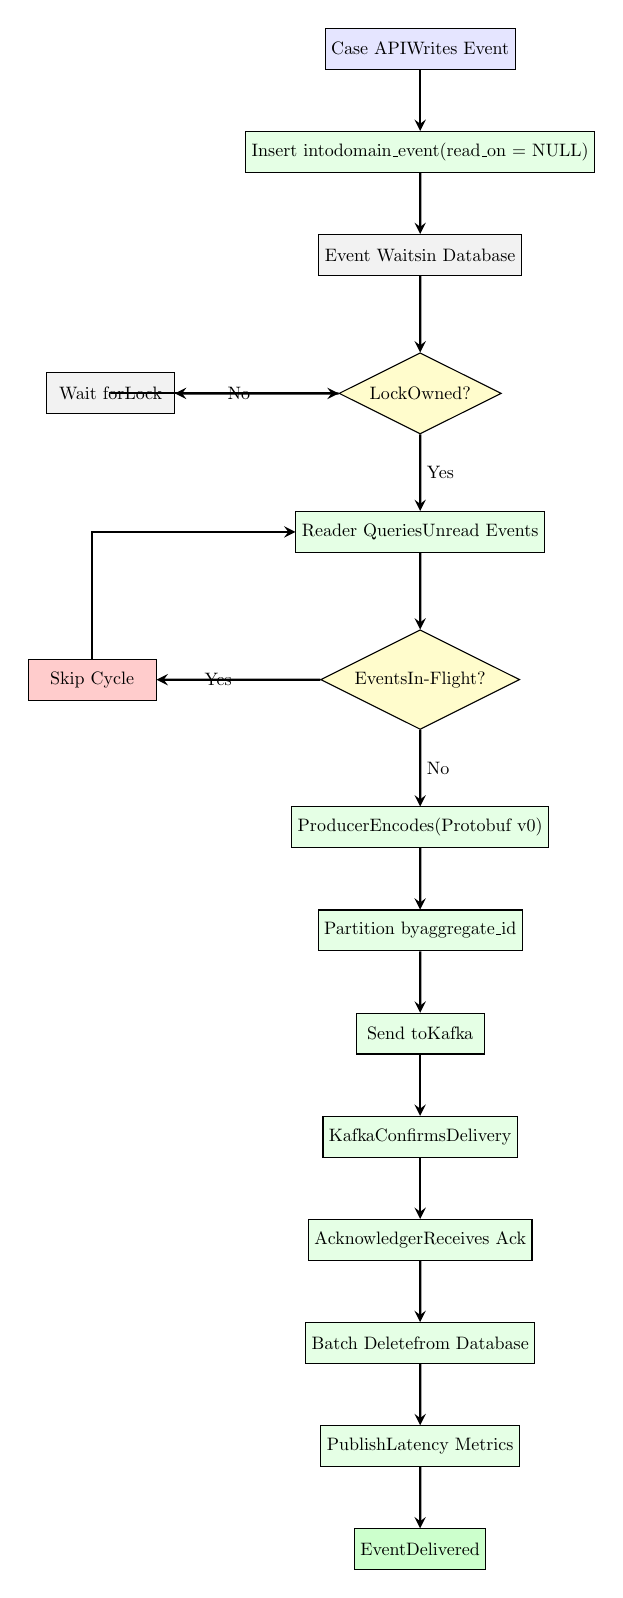
\begin{tikzpicture}[node distance=1.2cm, scale=0.65, every node/.style={transform shape}]

% Start
\node (api-write) [process, fill=blue!10] {Case API\\Writes Event};

\node (db-insert) [process, below=of api-write] {Insert into\\domain\_event\\(read\_on = NULL)};

\node (wait) [process, below=of db-insert, fill=gray!10] {Event Waits\\in Database};

% Lock check
\node (lock-check) [decision, below=of wait, yshift=-0.3cm] {Lock\\Owned?};

\node (wait-lock) [process, left=of lock-check, xshift=-2cm, fill=gray!10] {Wait for\\Lock};

% Read
\node (read) [process, below=of lock-check, yshift=-0.3cm] {Reader Queries\\Unread Events};

\node (in-flight-check) [decision, below=of read, yshift=-0.3cm] {Events\\In-Flight?};

\node (skip) [process, left=of in-flight-check, xshift=-2cm, fill=red!20] {Skip Cycle};

% Produce
\node (encode) [process, below=of in-flight-check, yshift=-0.3cm] {Producer\\Encodes\\(Protobuf v0)};

\node (partition) [process, below=of encode] {Partition by\\aggregate\_id};

\node (kafka-send) [process, below=of partition] {Send to\\Kafka};

% Kafka ack
\node (kafka-ack) [process, below=of kafka-send] {Kafka\\Confirms\\Delivery};

\node (ack-received) [process, below=of kafka-ack] {Acknowledger\\Receives Ack};

\node (batch-delete) [process, below=of ack-received] {Batch Delete\\from Database};

\node (metrics-pub) [process, below=of batch-delete] {Publish\\Latency Metrics};

\node (done) [process, fill=green!20, below=of metrics-pub] {Event\\Delivered};

% Arrows
\draw [arrow] (api-write) -- (db-insert);
\draw [arrow] (db-insert) -- (wait);
\draw [arrow] (wait) -- (lock-check);
\draw [arrow] (lock-check) -- node[left] {No} (wait-lock);
\draw [arrow] (wait-lock) |- (lock-check);
\draw [arrow] (lock-check) -- node[right] {Yes} (read);
\draw [arrow] (read) -- (in-flight-check);
\draw [arrow] (in-flight-check) -- node[left] {Yes} (skip);
\draw [arrow] (skip) |- (read);
\draw [arrow] (in-flight-check) -- node[right] {No} (encode);
\draw [arrow] (encode) -- (partition);
\draw [arrow] (partition) -- (kafka-send);
\draw [arrow] (kafka-send) -- (kafka-ack);
\draw [arrow] (kafka-ack) -- (ack-received);
\draw [arrow] (ack-received) -- (batch-delete);
\draw [arrow] (batch-delete) -- (metrics-pub);
\draw [arrow] (metrics-pub) -- (done);

\end{tikzpicture}
\caption{Event Processing Flow}
\end{figure}

\clearpage

\section{Lock Management}

The distributed lock mechanism ensures only one pod processes events at a time, preventing duplicate deliveries while enabling high availability.

\begin{figure}[H]
\centering
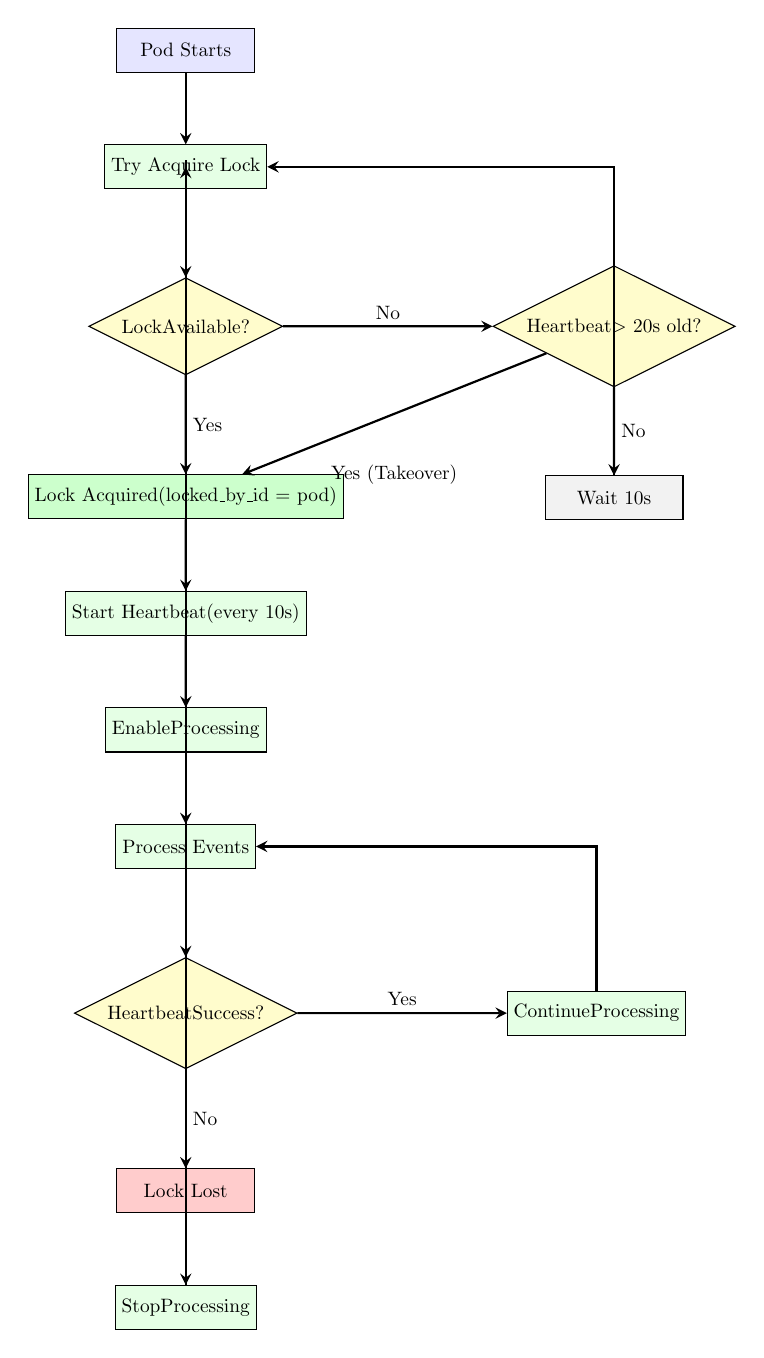
\begin{tikzpicture}[node distance=1.3cm, scale=0.7, every node/.style={transform shape}]

% Pod startup
\node (start) [process, fill=blue!10] {Pod Starts};

\node (try-lock) [process, below=of start] {Try Acquire Lock};

\node (lock-check) [decision, below=of try-lock, yshift=-0.3cm] {Lock\\Available?};

% Lock unavailable path
\node (check-heartbeat) [decision, right=of lock-check, xshift=2.5cm] {Heartbeat\\$>$ 20s old?};

\node (wait) [process, below=of check-heartbeat, yshift=-0.3cm, fill=gray!10] {Wait 10s};

% Lock acquired path
\node (lock-acquired) [process, below=of lock-check, yshift=-0.5cm, fill=green!20] {Lock Acquired\\(locked\_by\_id = pod)};

\node (start-heartbeat) [process, below=of lock-acquired] {Start Heartbeat\\(every 10s)};

\node (start-processing) [process, below=of start-heartbeat] {Enable\\Processing};

% Processing loop
\node (process-events) [process, below=of start-processing] {Process Events};

\node (heartbeat-ok) [decision, below=of process-events, yshift=-0.3cm] {Heartbeat\\Success?};

% Heartbeat success
\node (continue) [process, right=of heartbeat-ok, xshift=2.5cm] {Continue\\Processing};

% Heartbeat failure
\node (lock-lost) [process, below=of heartbeat-ok, yshift=-0.5cm, fill=red!20] {Lock Lost};

\node (stop-processing) [process, below=of lock-lost] {Stop\\Processing};

% Arrows
\draw [arrow] (start) -- (try-lock);
\draw [arrow] (try-lock) -- (lock-check);
\draw [arrow] (lock-check) -- node[above] {No} (check-heartbeat);
\draw [arrow] (check-heartbeat) -- node[right] {No} (wait);
\draw [arrow] (wait) |- (try-lock);
\draw [arrow] (check-heartbeat) -- node[below, yshift=-0.8cm] {Yes (Takeover)} (lock-acquired);
\draw [arrow] (lock-check) -- node[right] {Yes} (lock-acquired);
\draw [arrow] (lock-acquired) -- (start-heartbeat);
\draw [arrow] (start-heartbeat) -- (start-processing);
\draw [arrow] (start-processing) -- (process-events);
\draw [arrow] (process-events) -- (heartbeat-ok);
\draw [arrow] (heartbeat-ok) -- node[above] {Yes} (continue);
\draw [arrow] (continue) |- (process-events);
\draw [arrow] (heartbeat-ok) -- node[right] {No} (lock-lost);
\draw [arrow] (lock-lost) -- (stop-processing);
\draw [arrow] (stop-processing) |- (try-lock);

\end{tikzpicture}
\caption{Lock Acquisition and Maintenance}
\end{figure}

\subsection{Lock Behavior}

\textbf{Acquisition Conditions}
\begin{itemize}
    \item Lock table has no entry OR
    \item Existing lock's \texttt{latest\_heartbeat\_at} is older than 2x heartbeat period (20 seconds)
    \item Prevents split-brain: 2x period ensures stale lock before takeover
\end{itemize}

\textbf{Heartbeat Mechanism}
\begin{itemize}
    \item Updates \texttt{latest\_heartbeat\_at} every 10 seconds
    \item Must verify current ownership (locked\_by\_id matches pod ID)
    \item Failed heartbeat immediately stops event processing
    \item Grace period: 20 seconds for failover
\end{itemize}

\textbf{Failover Scenario}
\begin{enumerate}
    \item Active pod crashes or becomes unresponsive
    \item Heartbeat stops updating
    \item After 20 seconds, standby pod detects stale heartbeat
    \item Standby pod acquires lock
    \item New owner begins processing within 10 seconds (next heartbeat cycle)
    \item Total failover time: 20-30 seconds
\end{enumerate}

\clearpage

\section{Database Integration}

\subsection{Schema Overview}

\textbf{domain\_event Table}

\begin{lstlisting}[language=SQL,basicstyle=\small\ttfamily]
CREATE TABLE domain_event (
    id                   BIGSERIAL PRIMARY KEY,
    aggregate_id         UUID NOT NULL,
    event_type           TEXT NOT NULL,
    wire                 BYTEA NOT NULL,
    read_on              TIMESTAMP,
    written_at           TIMESTAMP NOT NULL DEFAULT NOW(),
    is_dirty             BOOLEAN NOT NULL DEFAULT FALSE,
    org_id               BIGINT NOT NULL,
    aggregate_version    BIGINT NOT NULL
);

CREATE INDEX domain_event_scrapper_idx
ON domain_event (written_at DESC, aggregate_version DESC)
WHERE read_on IS NULL AND is_dirty IS FALSE;
\end{lstlisting}

\textbf{Column Descriptions}
\begin{itemize}
    \item \texttt{id}: Unique event identifier (auto-increment)
    \item \texttt{aggregate\_id}: Entity UUID (case, project, etc.) - used for Kafka partitioning
    \item \texttt{event\_type}: Domain event type (CaseCreated, StatusChanged, etc.)
    \item \texttt{wire}: Protobuf-encoded event payload
    \item \texttt{read\_on}: Timestamp when event was read (NULL = unread)
    \item \texttt{written\_at}: Event creation timestamp
    \item \texttt{is\_dirty}: Flag for corrupt/unprocessable events
    \item \texttt{org\_id}: Organization identifier for multi-tenancy
    \item \texttt{aggregate\_version}: Entity version for optimistic locking
\end{itemize}

\textbf{event\_relay\_lock Table}

\begin{lstlisting}[language=SQL,basicstyle=\small\ttfamily]
CREATE TABLE event_relay_lock (
    latest_heartbeat_at  TIMESTAMP NOT NULL,
    locked_by_id         TEXT NOT NULL
);

-- Single row table (enforced by application logic)
\end{lstlisting}

\textbf{Column Descriptions}
\begin{itemize}
    \item \texttt{latest\_heartbeat\_at}: Last successful heartbeat timestamp
    \item \texttt{locked\_by\_id}: Pod identifier of current lock owner
\end{itemize}

\subsection{Query Patterns}

\textbf{Read Unread Events}
\begin{lstlisting}[language=SQL,basicstyle=\small\ttfamily]
SELECT id, aggregate_id, event_type, wire, org_id, written_at
FROM domain_event
WHERE read_on IS NULL
  AND is_dirty IS FALSE
  AND EXISTS (
      SELECT 1 FROM event_relay_lock
      WHERE locked_by_id = $1 -- current pod ID
        AND latest_heartbeat_at > NOW() - INTERVAL '20 seconds'
  )
ORDER BY written_at ASC, aggregate_version ASC
LIMIT 1000;
\end{lstlisting}

\textbf{Batch Delete Acknowledged Events}
\begin{lstlisting}[language=SQL,basicstyle=\small\ttfamily]
DELETE FROM domain_event
WHERE id = ANY($1::BIGINT[]);
-- $1 is array of up to 1000 event IDs
\end{lstlisting}

\textbf{Mark Corrupt Events as Dirty}
\begin{lstlisting}[language=SQL,basicstyle=\small\ttfamily]
UPDATE domain_event
SET is_dirty = TRUE
WHERE id = ANY($1::BIGINT[]);
\end{lstlisting}

\textbf{Count Unread Events}
\begin{lstlisting}[language=SQL,basicstyle=\small\ttfamily]
SELECT COUNT(*)
FROM domain_event
WHERE read_on IS NULL AND is_dirty IS FALSE;
\end{lstlisting}

\subsection{Performance Optimizations}

\begin{itemize}
    \item \textbf{Index}: Partial index on (written\_at DESC, aggregate\_version DESC) where unread and not dirty
    \item \textbf{Connection Pool}: 10 max connections (idle and open)
    \item \textbf{Batch Operations}: Deletes up to 1000 events per transaction
    \item \textbf{Lock Verification}: Embedded in read query for atomic ownership check
    \item \textbf{Dirty Flag}: Prevents repeated processing of corrupt events
\end{itemize}

\clearpage

\section{Kafka Integration}

\subsection{Producer Configuration}

\begin{lstlisting}[basicstyle=\small\ttfamily]
[dd.kafka.producer]
topic = domain-events                # Case Management tenant
partition_count = 32                 # Number of partitions
linger_ms = 10                       # Batching delay
ack_timeout_ms = 100                 # Ack wait timeout
compression_codec = snappy           # Message compression
max_in_flight_requests = 5           # Parallel requests
idempotence = true                   # Exactly-once semantics
\end{lstlisting}

\subsection{Partitioning Strategy}

Events are partitioned by \texttt{aggregate\_id} (UUID) to ensure ordering guarantees:

\begin{lstlisting}[language=Go,basicstyle=\small\ttfamily]
partition := int(aggregate_id.ID()) % partition_count

// Example:
// aggregate_id = "550e8400-e29b-41d4-a716-446655440000"
// partition_count = 32
// partition = hash(UUID) % 32 = 17
\end{lstlisting}

\textbf{Benefits}
\begin{itemize}
    \item All events for a case/project go to the same partition
    \item Maintains event ordering per aggregate
    \item Enables parallel processing across partitions
    \item Simplifies downstream consumer state management
\end{itemize}

\subsection{Message Format}

Messages are protobuf-encoded with a version prefix:

\begin{lstlisting}[language=Go,basicstyle=\small\ttfamily]
// Wire format: [version_byte][protobuf_payload]
// version_byte = 0x00 (v0 encoding)

type KafkaMessage struct {
    Key       []byte  // aggregate_id as bytes
    Value     []byte  // version prefix + protobuf
    Headers   map[string]string {
        "trace.trace_id":  "12345...",
        "trace.span_id":   "67890...",
        "org_id":          "123456",
        "event_type":      "CaseCreated"
    }
}
\end{lstlisting}

\subsection{Topics and Tenants}

\begin{table}[H]
\centering
\caption{Kafka Topics by Tenant}
\begin{tabularx}{\textwidth}{|l|X|X|}
\hline
\textbf{Topic} & \textbf{Tenant} & \textbf{Purpose} \\
\hline
domain-events & case-management & Case Management domain events \\
\hline
domain-events-oncall & on-call & On-Call product domain events \\
\hline
\end{tabularx}
\end{table}

\subsection{Event Types}

Over 60 domain event types are relayed through Kafka:

\begin{multicols}{2}
\small
\begin{itemize}
    \item CaseCreated
    \item CaseDeleted
    \item CaseArchived
    \item CaseUnarchived
    \item StatusChanged
    \item PriorityChanged
    \item TitleChanged
    \item DescriptionChanged
    \item CaseAssigned
    \item CaseUnassigned
    \item CommentAdded
    \item CommentUpdated
    \item CommentDeleted
    \item AttachmentCreated
    \item AttachmentDeleted
    \item JiraIssueAdded
    \item JiraIssueRemoved
    \item ServiceNowTicketAdded
    \item ServiceNowTicketRemoved
    \item IncidentLinked
    \item IncidentUnlinked
    \item AutomationRuleCreated
    \item AutomationRuleUpdated
    \item AutomationRuleEnabled
    \item AutomationRuleDisabled
    \item CellCreated
    \item LinkCreated
    \item LinkDeleted
    \item InsightsAdded
    \item InsightsRemoved
    \item ProjectUpdated
    \item ProjectDeleted
    \item [...and 28 more]
\end{itemize}
\end{multicols}

\clearpage

\section{Datacenter Deployment Strategy}

\subsection{Multi-Environment Deployment}

\begin{figure}[H]
\centering
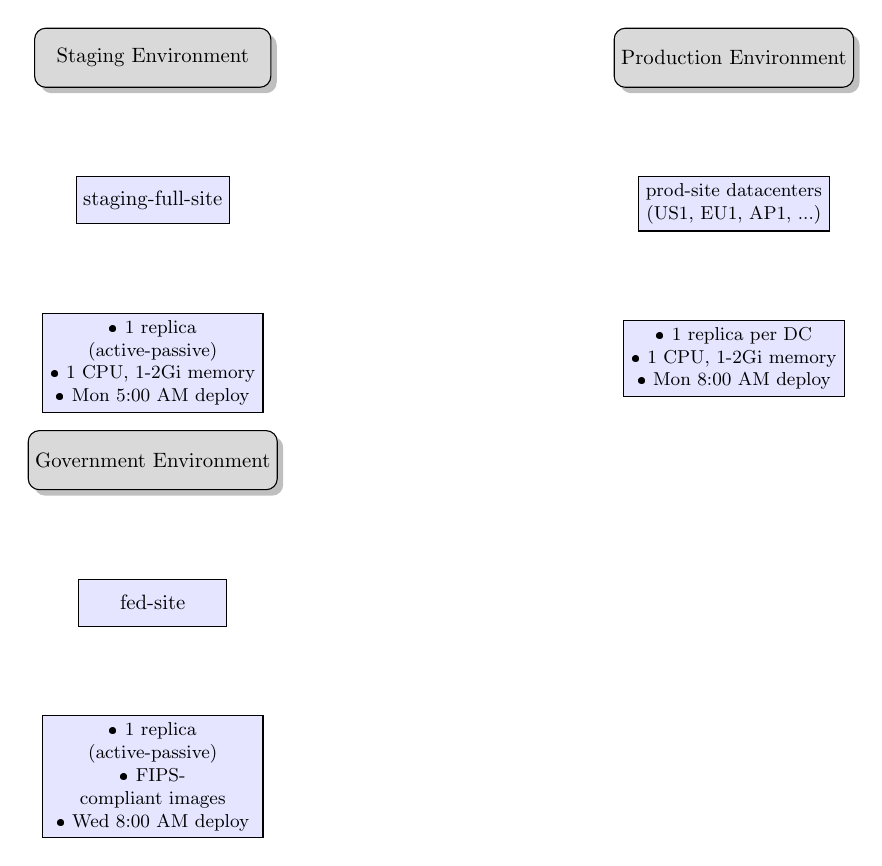
\begin{tikzpicture}[node distance=1.8cm, scale=0.75, every node/.style={transform shape}]

% Staging
\node (staging) [system, minimum width=4cm] {Staging Environment};
\node (staging-dc) [component, below=of staging, yshift=0.3cm] {staging-full-site};
\node (staging-details) [component, below=of staging-dc, yshift=0.3cm, text width=3.5cm, font=\small] {
    • 1 replica (active-passive)\\
    • 1 CPU, 1-2Gi memory\\
    • Mon 5:00 AM deploy
};

% Production
\node (prod) [system, minimum width=4cm, right=of staging, xshift=4cm] {Production Environment};
\node (prod-dcs) [component, below=of prod, yshift=0.3cm, text width=3cm, font=\small] {
    prod-site datacenters\\
    (US1, EU1, AP1, ...)
};
\node (prod-details) [component, below=of prod-dcs, yshift=0.3cm, text width=3.5cm, font=\small] {
    • 1 replica per DC\\
    • 1 CPU, 1-2Gi memory\\
    • Mon 8:00 AM deploy
};

% Government
\node (gov) [system, minimum width=4cm, below=of staging, yshift=-4cm] {Government Environment};
\node (gov-dc) [component, below=of gov, yshift=0.3cm] {fed-site};
\node (gov-details) [component, below=of gov-dc, yshift=0.3cm, text width=3.5cm, font=\small] {
    • 1 replica (active-passive)\\
    • FIPS-compliant images\\
    • Wed 8:00 AM deploy
};

\end{tikzpicture}
\caption{Deployment Strategy Across Environments}
\end{figure}

\subsection{Deployment Configuration}

\begin{table}[H]
\centering
\caption{Deployment Settings by Environment}
\begin{tabularx}{\textwidth}{|l|X|X|X|}
\hline
\textbf{Setting} & \textbf{Staging} & \textbf{Production} & \textbf{Government} \\
\hline
Datacenters & staging-full-site & prod-site (multiple) & fed-site \\
\hline
Replicas & 1 & 1 per DC & 1 \\
\hline
Active Pods & 1 (via lock) & 1 per DC (via lock) & 1 (via lock) \\
\hline
Deployment Strategy & RollingUpdate & RollingUpdate & RollingUpdate \\
\hline
Max Surge & 1 & 1 & 1 \\
\hline
Max Unavailable & 0 & 0 & 0 \\
\hline
CPU Request/Limit & 1 / 1 & 1 / 1 & 1 / 1 \\
\hline
Memory Request/Limit & 1Gi / 2Gi & 1Gi / 2Gi & 1Gi / 2Gi \\
\hline
Image & caseeventrelay & caseeventrelay & caseeventrelayfips \\
\hline
Schedule & Mon 5:00 AM & Mon 8:00 AM & Wed 8:00 AM \\
\hline
Health Gates & Basic monitoring & 20min health check & 20min health check \\
\hline
\end{tabularx}
\end{table}

\subsection{High Availability Strategy}

\textbf{Active-Passive Model}
\begin{itemize}
    \item Multiple replicas deployed per datacenter
    \item Only one replica actively processes events (lock owner)
    \item Other replicas act as warm standbys
    \item Automatic failover within 20-30 seconds on pod failure
    \item No event duplication due to distributed lock
\end{itemize}

\textbf{Zero-Downtime Deployments}
\begin{itemize}
    \item RollingUpdate strategy with maxSurge: 1, maxUnavailable: 0
    \item New pod starts and attempts lock acquisition
    \item Old pod maintains lock until termination
    \item Lock gracefully transfers during pod shutdown
    \item Minimal event processing interruption (sub-second)
\end{itemize}

\textbf{Health Checks}
\begin{itemize}
    \item Liveness Probe: /liveness on port 8080 (15s period, 3 failure threshold)
    \item Readiness Probe: /readiness on port 8080 (10s period, 3 failure threshold)
    \item Termination Grace Period: 30 seconds for graceful shutdown
\end{itemize}

\clearpage

\section{Performance and Observability}

\subsection{Key Metrics Collected}

\textbf{Event Processing Metrics}

\begin{lstlisting}[basicstyle=\small\ttfamily]
dd.case-event-relay.reads (count)
Tags: success:true/false
Description: Number of events read from database

dd.case-event-relay.acks (count)
Description: Number of events acknowledged and deleted

dd.case-event-relay.marked_dirty (count)
Description: Number of corrupt events marked as dirty

dd.case-event-relay.latency_ms (distribution)
Tags: kafka_partition
Description: End-to-end latency from written_at to Kafka ack
\end{lstlisting}

\textbf{System Health Metrics}

\begin{lstlisting}[basicstyle=\small\ttfamily]
dd.case-event-relay.unread_events (gauge)
Description: Count of unread events in database
Purpose: Backlog monitoring and alerting

dd.case-event-relay.is_lock_owner (gauge)
Values: 0 or 1
Description: Lock ownership status
Purpose: Active pod identification
\end{lstlisting}

\textbf{Database Metrics}

\begin{lstlisting}[basicstyle=\small\ttfamily]
dd.case.pg.query_duration (distribution)
Tags: query_name, success
Description: Database query latency

dd.case.pg.connection_pool.idle_connections (gauge)
dd.case.pg.connection_pool.open_connections (gauge)
Description: Connection pool health
\end{lstlisting}

\subsection{Dashboards}

\textbf{Production Dashboard}
\begin{itemize}
    \item URL: \url{https://app.datadoghq.com/dashboard/cq2-3tg-f2t}
    \item Panels: Throughput, latency percentiles, unread events, lock ownership, error rates
\end{itemize}

\textbf{Staging Dashboard}
\begin{itemize}
    \item URL: \url{https://ddstaging.datadoghq.com/dashboard/vbh-qu6-ydn}
\end{itemize}

\subsection{Tracing}

\textbf{APM Integration}
\begin{itemize}
    \item Service: case-event-relay
    \item Trace Propagation: Maintains context from original API request through Kafka
    \item Key Spans:
    \begin{itemize}
        \item \texttt{acknowledger.main\_loop} - Ack processing
        \item \texttt{process\_events} - Main processing loop
        \item \texttt{reader.read} - Database reads
        \item \texttt{producer.produce} - Kafka production
        \item \texttt{domain\_events\_repo.*} - Repository operations
    \end{itemize}
\end{itemize}

\subsection{Alerting}

\textbf{Critical Alerts}

\begin{enumerate}
    \item \textbf{High Backlog}
    \begin{itemize}
        \item Metric: \texttt{dd.case-event-relay.unread\_events}
        \item Threshold: $>$ 10,000 events for $>$ 10 minutes
        \item Indicates: Throughput issue or downstream Kafka problem
    \end{itemize}

    \item \textbf{No Lock Owner}
    \begin{itemize}
        \item Metric: \texttt{dd.case-event-relay.is\_lock\_owner}
        \item Threshold: Sum across all pods = 0 for $>$ 2 minutes
        \item Indicates: All pods unable to acquire lock (database issue)
    \end{itemize}

    \item \textbf{High Latency}
    \begin{itemize}
        \item Metric: \texttt{dd.case-event-relay.latency\_ms (p99)}
        \item Threshold: $>$ 5 seconds for $>$ 5 minutes
        \item Indicates: Database or Kafka performance degradation
    \end{itemize}

    \item \textbf{High Dirty Event Rate}
    \begin{itemize}
        \item Metric: \texttt{dd.case-event-relay.marked\_dirty}
        \item Threshold: $>$ 10 events per minute for $>$ 5 minutes
        \item Indicates: Data corruption or protobuf schema issues
    \end{itemize}
\end{enumerate}

\clearpage

\section{Reliability Patterns}

\subsection{Transactional Outbox Pattern}

The service implements the transactional outbox pattern to ensure reliable event delivery:

\textbf{Benefits}
\begin{itemize}
    \item Events stored in same database transaction as domain changes
    \item Database ACID properties guarantee event persistence
    \item Events only deleted after Kafka confirms delivery
    \item No message loss on relay service failures
    \item At-least-once delivery semantics
\end{itemize}

\textbf{Implementation}
\begin{enumerate}
    \item Case API writes event to \texttt{domain\_event} table in same transaction as business logic
    \item Event relay reads unread events
    \item Event relay publishes to Kafka
    \item Kafka confirms delivery
    \item Event relay deletes event from database
    \item If any step fails, event remains in database for retry
\end{enumerate}

\subsection{Active-Passive High Availability}

\textbf{Design Principles}
\begin{itemize}
    \item Single active processor prevents duplicate deliveries
    \item Multiple replicas provide failover capability
    \item Distributed lock coordinates across replicas
    \item Automatic failover on active pod failure
    \item No split-brain due to 2x heartbeat grace period
\end{itemize}

\textbf{Failure Scenarios}

\textit{Active Pod Crashes}
\begin{enumerate}
    \item Active pod stops heartbeating
    \item After 20 seconds, standby detects stale heartbeat
    \item Standby acquires lock
    \item Standby begins processing
    \item Unread events processed normally
    \item Recovery time: 20-30 seconds
\end{enumerate}

\textit{Database Connection Loss}
\begin{enumerate}
    \item Read/heartbeat operations fail
    \item Lock ownership lost
    \item Processing stops
    \item Connection pool attempts reconnection
    \item On reconnect, attempt lock reacquisition
    \item Processing resumes
\end{enumerate}

\textit{Kafka Producer Failure}
\begin{enumerate}
    \item Kafka client throws error
    \item Events remain in database (not deleted)
    \item Kafka client auto-reconnects
    \item Next read cycle retries undelivered events
    \item Events delivered with slightly higher latency
    \item Potential duplicate deliveries (at-least-once semantics)
\end{enumerate}

\subsection{Corrupt Event Handling}

\textbf{Detection and Isolation}
\begin{itemize}
    \item Protobuf decode errors during read
    \item Invalid event structure or missing required fields
    \item Events marked with \texttt{is\_dirty = TRUE}
    \item Dirty events excluded from future reads
    \item Prevents pipeline blocking on single corrupt event
    \item Manual investigation and remediation required
\end{itemize}

\textbf{Monitoring}
\begin{itemize}
    \item Metric: \texttt{dd.case-event-relay.marked\_dirty}
    \item Alert on sustained dirty event rate
    \item Dashboards show dirty event counts over time
\end{itemize}

\subsection{Backpressure Management}

\textbf{In-Flight Event Protection}
\begin{itemize}
    \item Processor checks for in-flight events before reading
    \item Only one batch processed at a time
    \item Prevents overwhelming Kafka producer
    \item Ensures ordered delivery within partitions
    \item Simple but effective flow control
\end{itemize}

\textbf{Batch Sizing}
\begin{itemize}
    \item Read batch: 1000 events max
    \item Ack batch: 1000 events max
    \item Tuned for throughput vs memory usage balance
    \item Prevents large transaction contention in PostgreSQL
\end{itemize}

\clearpage

\section{Technical Implementation Details}

\subsection{Core Components}

\textbf{Main Entry Point} (\texttt{main.go})

\begin{lstlisting}[language=Go,basicstyle=\small\ttfamily]
func main() {
    // Initialize database connection
    db := initDB()
    repo := domainevent.NewRepository(db)

    // Initialize Kafka producer
    producer := initKafkaProducer()

    // Create components
    lockCtrl := NewLockController(repo)
    reader := NewReader(repo)
    kafkaProducer := NewProducer(producer)
    acknowledger := NewAcknowledger(repo)
    metricsGen := NewMetricsGenerator(repo)
    processor := NewProcessor(
        lockCtrl, reader, kafkaProducer, acknowledger
    )

    // Start goroutines
    go lockCtrl.Run(ctx)
    go processor.Run(ctx)
    go acknowledger.Run(ctx)
    go metricsGen.Run(ctx)

    // Health check server
    http.HandleFunc("/liveness", livenessHandler)
    http.HandleFunc("/readiness", readinessHandler)
    http.ListenAndServe(":8080", nil)
}
\end{lstlisting}

\textbf{LockController} (\texttt{lock\_controller.go})

\begin{lstlisting}[language=Go,basicstyle=\small\ttfamily]
type LockController struct {
    repo            *domainevent.Repository
    heartbeatPeriod time.Duration // 10 seconds
    podID           string
    isOwner         atomic.Bool
}

func (lc *LockController) Run(ctx context.Context) {
    ticker := time.NewTicker(lc.heartbeatPeriod)
    for {
        select {
        case <-ticker.C:
            if lc.isOwner.Load() {
                err := lc.repo.HeartBeatTheLock(lc.podID)
                if err != nil {
                    lc.isOwner.Store(false)
                }
            } else {
                err := lc.repo.TryToAcquireTheLock(lc.podID)
                if err == nil {
                    lc.isOwner.Store(true)
                }
            }
        case <-ctx.Done():
            return
        }
    }
}
\end{lstlisting}

\textbf{Processor} (\texttt{processor.go})

\begin{lstlisting}[language=Go,basicstyle=\small\ttfamily]
type Processor struct {
    lockCtrl    *LockController
    reader      *Reader
    producer    *Producer
    pollingPeriod time.Duration // 250ms
    inFlight    atomic.Bool
}

func (p *Processor) Run(ctx context.Context) {
    ticker := time.NewTicker(p.pollingPeriod)
    for {
        select {
        case <-ticker.C:
            if !p.lockCtrl.IsOwner() {
                continue
            }
            if p.inFlight.Load() {
                continue
            }

            p.inFlight.Store(true)
            events, err := p.reader.Read(ctx)
            if err != nil {
                p.inFlight.Store(false)
                continue
            }

            for _, event := range events {
                p.producer.Produce(event)
            }

            // Note: inFlight cleared by acknowledger
        case <-ctx.Done():
            return
        }
    }
}
\end{lstlisting}

\textbf{Acknowledger} (\texttt{acknowledger.go})

\begin{lstlisting}[language=Go,basicstyle=\small\ttfamily]
type Acknowledger struct {
    repo       *domainevent.Repository
    ackChan    chan *Ack
    batchSize  int           // 1000
    tickPeriod time.Duration // 20ms
}

func (a *Acknowledger) Run(ctx context.Context) {
    ticker := time.NewTicker(a.tickPeriod)
    batch := make([]*Ack, 0, a.batchSize)

    for {
        select {
        case ack := <-a.ackChan:
            batch = append(batch, ack)
            if len(batch) >= a.batchSize {
                a.processBatch(batch)
                batch = batch[:0]
            }
        case <-ticker.C:
            if len(batch) > 0 {
                a.processBatch(batch)
                batch = batch[:0]
            }
        case <-ctx.Done():
            return
        }
    }
}

func (a *Acknowledger) processBatch(batch []*Ack) {
    ids := extractIDs(batch)
    err := a.repo.BatchDelete(ids)
    if err == nil {
        for _, ack := range batch {
            latency := time.Since(ack.WrittenAt)
            metrics.Distribution(
                "latency_ms",
                float64(latency.Milliseconds()),
                "kafka_partition", ack.Partition,
            )
        }
    }
}
\end{lstlisting}

\subsection{Concurrency Model}

\begin{itemize}
    \item \textbf{Goroutines}: 4 main goroutines (LockController, Processor, Acknowledger, MetricsGenerator)
    \item \textbf{Synchronization}: Atomic booleans for lock ownership and in-flight state
    \item \textbf{Channels}: Kafka ack channel for asynchronous acknowledgment
    \item \textbf{Context}: Used for graceful shutdown across all goroutines
    \item \textbf{Stopper Pattern}: Coordinates shutdown sequence
\end{itemize}

\subsection{Dependencies}

\textbf{Key Go Dependencies}
\begin{itemize}
    \item \texttt{github.com/confluentinc/confluent-kafka-go/kafka} - Kafka client
    \item \texttt{github.com/lib/pq} - PostgreSQL driver
    \item \texttt{google.golang.org/protobuf} - Protobuf encoding
    \item \texttt{gopkg.in/DataDog/dd-trace-go.v1} - Distributed tracing
    \item \texttt{github.com/DataDog/datadog-go/statsd} - Metrics
\end{itemize}

\clearpage

\section{Operational Considerations}

\subsection{Scalability}

\textbf{Current Model}
\begin{itemize}
    \item Single active processor per datacenter
    \item Throughput limited by single-threaded read-produce cycle
    \item Sufficient for current case management load ($<$ 10k events/sec)
    \item Kafka partitioning enables downstream parallel processing
\end{itemize}

\textbf{Scaling Options}

\textit{Vertical Scaling}
\begin{itemize}
    \item Increase CPU/memory allocation
    \item Increase batch sizes (read and ack)
    \item Tune polling period for higher frequency
    \item Limited by single-pod processing model
\end{itemize}

\textit{Horizontal Scaling (Future)}
\begin{itemize}
    \item Partition \texttt{domain\_event} table by org\_id or hash
    \item Run multiple relay instances per partition
    \item Requires schema changes and migration
    \item Enables 10x+ throughput increase
\end{itemize}

\subsection{Monitoring Best Practices}

\textbf{Daily Checks}
\begin{itemize}
    \item Monitor \texttt{unread\_events} gauge (should be near zero)
    \item Check \texttt{latency\_ms p99} (should be $<$ 1 second)
    \item Verify \texttt{is\_lock\_owner} sum = 1 per datacenter
    \item Review dirty event counts (should be zero)
\end{itemize}

\textbf{Incident Response}

\textit{High Backlog}
\begin{enumerate}
    \item Check Kafka producer health (metrics, logs)
    \item Verify lock ownership (multiple owners = split-brain)
    \item Check database query latency
    \item Review recent case-api deployment (event surge)
    \item Consider temporary batch size increase
\end{enumerate}

\textit{No Active Processor}
\begin{enumerate}
    \item Check all pods (kubectl get pods)
    \item Review pod logs for lock acquisition failures
    \item Verify database connectivity
    \item Check \texttt{event\_relay\_lock} table state
    \item Manual lock reset if needed (UPDATE event\_relay\_lock SET latest\_heartbeat\_at = '1970-01-01')
\end{enumerate}

\subsection{Maintenance Operations}

\textbf{Draining Events}
\begin{lstlisting}[language=SQL,basicstyle=\small\ttfamily]
-- Check unread event count
SELECT COUNT(*) FROM domain_event
WHERE read_on IS NULL AND is_dirty IS FALSE;

-- Monitor until count reaches zero
-- Safe to perform maintenance once drained
\end{lstlisting}

\textbf{Cleaning Dirty Events}
\begin{lstlisting}[language=SQL,basicstyle=\small\ttfamily]
-- Identify dirty events
SELECT id, aggregate_id, event_type, written_at
FROM domain_event
WHERE is_dirty IS TRUE
ORDER BY written_at DESC
LIMIT 100;

-- After investigation and remediation
DELETE FROM domain_event WHERE is_dirty IS TRUE;
\end{lstlisting}

\textbf{Manual Lock Reset}
\begin{lstlisting}[language=SQL,basicstyle=\small\ttfamily]
-- Emergency lock reset (if all pods deadlocked)
UPDATE event_relay_lock
SET latest_heartbeat_at = '1970-01-01 00:00:00';

-- Pods will detect stale heartbeat and compete for lock
\end{lstlisting}

\subsection{Service Catalog}

\begin{itemize}
    \item \textbf{Service}: case-event-relay
    \item \textbf{Team}: case-management
    \item \textbf{On-Call}: \url{https://app.datadoghq.com/on-call/teams/bc33b578-f8a9-11ed-a001-da7ad0900002}
    \item \textbf{Slack}: \#case-management
    \item \textbf{Repository}: \url{https://github.com/DataDog/dd-source/tree/main/domains/case_management/apps/case-event-relay}
    \item \textbf{Documentation}: \url{https://datadoghq.atlassian.net/wiki/spaces/CM/pages/3294330939/Case+Event+Relay}
\end{itemize}

\clearpage

\section{Future Considerations}

\subsection{Performance Enhancements}

\begin{itemize}
    \item \textbf{Table Partitioning}: Partition \texttt{domain\_event} by time range or hash for horizontal scaling
    \item \textbf{Read Optimization}: Materialized view for unread events to avoid index scan
    \item \textbf{Parallel Processing}: Multiple relay instances with partition-based work distribution
    \item \textbf{Compression}: Enable Kafka message compression for bandwidth reduction
    \item \textbf{Batch Tuning}: Dynamic batch sizing based on backlog depth
\end{itemize}

\subsection{Reliability Improvements}

\begin{itemize}
    \item \textbf{Dead Letter Queue}: Automatic routing of repeatedly failing events to DLQ
    \item \textbf{Circuit Breaker}: Kafka producer circuit breaker for graceful degradation
    \item \textbf{Health Scoring}: Composite health score for more nuanced monitoring
    \item \textbf{Auto-Recovery}: Automatic dirty event analysis and retry
\end{itemize}

\subsection{Operational Enhancements}

\begin{itemize}
    \item \textbf{Self-Service Metrics}: Per-org and per-event-type throughput dashboards
    \item \textbf{Canary Deployments}: Gradual rollout with synthetic event validation
    \item \textbf{Chaos Testing}: Automated fault injection for resilience validation
    \item \textbf{Lock Observability}: Detailed lock contention and handoff metrics
\end{itemize}

\section{Conclusion}

The Case-Event-Relay service serves as the critical bridge between the Case Management database and Kafka event streaming platform. Its implementation of the transactional outbox pattern ensures reliable, at-least-once delivery of domain events to downstream consumers while maintaining high availability through an active-passive deployment model.

\textbf{Key Architectural Strengths:}

\begin{itemize}
    \item \textbf{Reliability}: Transactional outbox pattern prevents event loss
    \item \textbf{High Availability}: Active-passive with automatic failover in 20-30 seconds
    \item \textbf{Ordering Guarantees}: Partition-by-aggregate ensures per-entity event ordering
    \item \textbf{Simplicity}: Single-threaded processing eliminates concurrency bugs
    \item \textbf{Observability}: Comprehensive metrics for latency, throughput, and backlog
    \item \textbf{Fault Isolation}: Dirty event marking prevents pipeline blocking
\end{itemize}

\textbf{Operational Excellence:}

\begin{itemize}
    \item \textbf{Zero-Downtime Deployments}: RollingUpdate with graceful lock handoff
    \item \textbf{Predictable Failover}: Well-defined 20-second lock timeout
    \item \textbf{Comprehensive Monitoring}: Metrics, tracing, and dashboards for all scenarios
    \item \textbf{Simple Troubleshooting}: Clear error paths and manual intervention procedures
\end{itemize}

\textbf{Integration Characteristics:}

\begin{itemize}
    \item \textbf{Database}: Direct PostgreSQL integration with connection pooling
    \item \textbf{Kafka}: OAuth-authenticated, TLS-encrypted, idempotent producer
    \item \textbf{Downstream}: Enables 10+ event handler flavors and third-party integrations
    \item \textbf{Tracing}: Full distributed tracing from API to consumer
\end{itemize}

The service's architecture prioritizes correctness and reliability over raw throughput. The active-passive model with distributed locking ensures exactly-one active processor, preventing duplicate event deliveries while enabling automatic failover on pod failures. The transactional outbox pattern guarantees no event loss, even during relay service failures. As Case Management scales, the architecture provides clear paths for horizontal scaling through table partitioning and parallel relay instances.

This report provides a comprehensive technical overview of the Case-Event-Relay service, its transactional outbox implementation, lock management strategy, and operational characteristics across Datadog's global infrastructure.

\vspace{1cm}

\hrule

\vspace{0.5cm}

\textit{This report documents the Case-Event-Relay service as of January 2026. For the latest implementation details, refer to the source code at:}

\texttt{domains/case\_management/apps/case-event-relay}

\end{document}
